\documentclass[10pt,a4paper]{report}
\usepackage[utf8]{inputenc}
\usepackage[english]{babel}
\usepackage{amsmath}
\usepackage{amsfonts}
\usepackage{amssymb}
\usepackage{graphicx}
\usepackage[left=2cm,right=2cm,top=2cm,bottom=2cm]{geometry}
\usepackage[autostyle, italian=quotes]{csquotes}
\usepackage{hyperref}
\author{Daniele Gilio}
\title{Exam Assignment}
\begin{document}
\maketitle
\section{Introduction}
This assignment was about text classification. We had to classify News titles by their topic; our classes were \enquote{science}, \enquote{health}, \enquote{business} and \enquote{entertainment}. Our raw features were the title itself and the publisher. The dataset was already divided in $10000$ training samples, $1000$ validation samples and $1000$ test samples. Our objective is to create a feature extraction process and to build one or more classifiers.
\section{Feature Extraction}
Since we are dealing with text classification we chose to employ the Bag of Words representation to encode the titles. In order to do that we had to build a fixed size dictionary. In Figure \ref{fig:acc_vs_dic} we can see how the dictionary size affects the performance of the models we intend to build.
\begin{figure}[!ht]
\centering
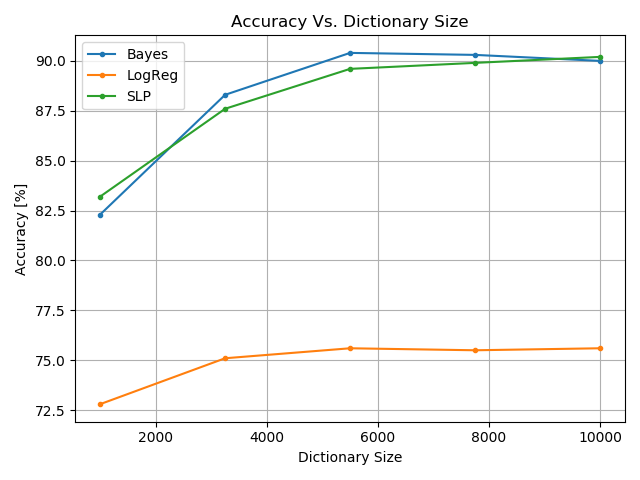
\includegraphics[width=0.5\linewidth]{acc_vs_dic.png}
\caption{Test Accuracy vs. Dictionary Size}
\label{fig:acc_vs_dic}
\end{figure}
Our goal with Figure \ref{fig:acc_vs_dic} was not to find the optimal dictionary size but to see if a bigger dictionary implied a better performance and this seems to be the case. Another decision we had to make was choosing if the publisher was a useful feature to keep. 
\begin{figure}[!ht]
\centering
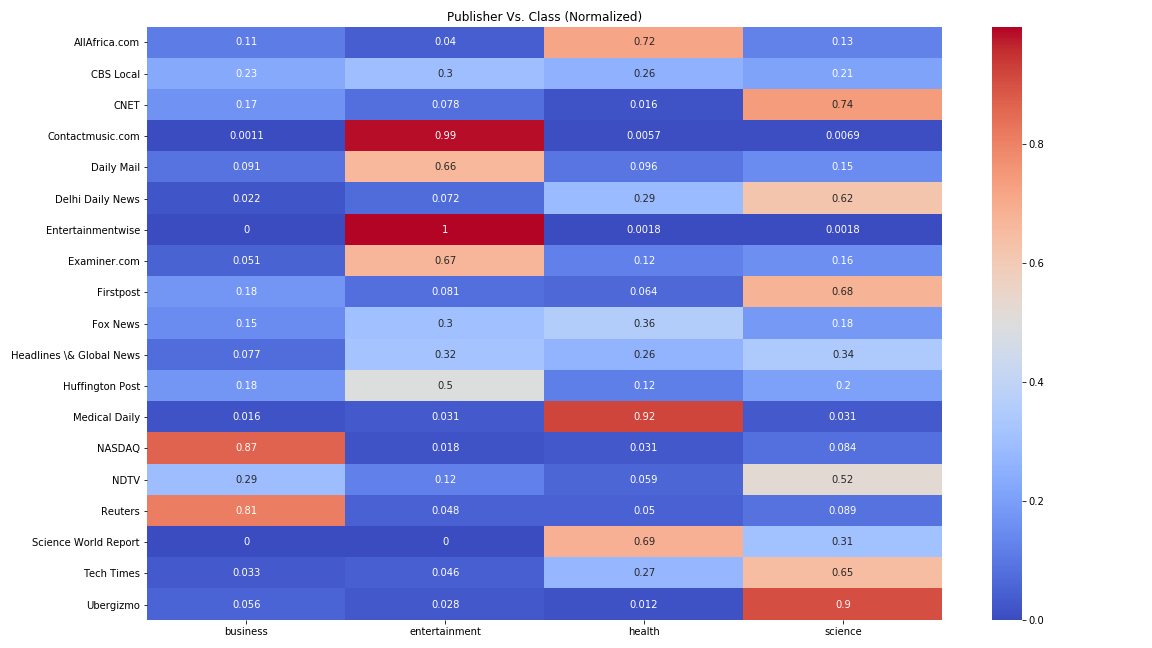
\includegraphics[width=0.8\linewidth]{pub_vs_class.png}
\caption{Publisher Class Distribution}
\label{fig:pub_vs_class}
\end{figure}
As we can see from Figure \ref{fig:pub_vs_class}, the $19$ different publishers mostly belong to a couple of classes. Based on that information we decide to keep the publisher information and we concatenated it to the title BoW. The simplest solution we found to encode the publishers was just to number them from $0$ to $18$. We also took into consideration normalization techniques, both in terms of words normalization (remove common words from the dictionary and stemming) and BoW normalization. We found out that using only one word normalization technique worsened the performance of all the models but using them both made them perform better. That said we used word normalization techniques for all the test we performed. Each model reacted differently to different BoW normalizations so we will discuss them separately.  
\section{Classifiers}
We decided to build a total of $4$ classifiers: Multinomial Bayesian Classifier, Multinomial Logistic Regression, Single Layer Perceptron and Multi-Layer Perceptron. The first two choices were biased upon the results we obtained in the Sentiment Analysis assignment. The latter two were chosen because of their versatility and previous assignments results. To be completely honest we would have liked to use SVMs since they proved to be the best in text recognition but we cannot since we are dealing with a multi-class problem, we would need a sort of multinomial SVM for which we do not have the theoretical background nor any code ready to be used. We settled on a dictionary size of $8000$ words, as it is very close to the maximum possible size given the normalizations performed on the corpus.
\subsection{Multinomial Naive Bayesian Classifier}
We chose the \textit{Multinomial Bayesian Classifier} as our baseline for testing since it proved to be simple but effective. Its simplicity meant that we could run multiple tests without worrying about the computational time needed to train it. The results of this classifier caught us off guard and proved to be challenging to beat. The Multinomial Bayesian Classifier reacted poorly upon BoW Normalization. L1 and L2 nearly cut the test accuracy in half and MaxAbs lowered it by a couple of percentage points. With those results we chose not to use any normalization to let this classifier perform at its best. The training accuracy was $94.39 \%$, the validation one was $89.2 \%$ and the test one was $91.1 \%$.
\begin{figure}[!ht]
\centering
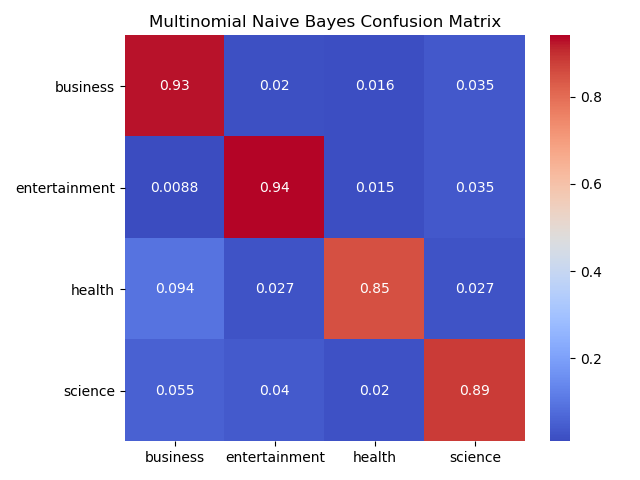
\includegraphics[width=0.5\linewidth]{bayes_confmat.png}
\caption{Bayesian Classifier Confusion Matrix (Test Set)}
\label{fig:bayes_confmat}
\end{figure}
\subsection{Multinomial Logistic Regression}
The \textit{Multinomial Logistic Regression} classifier was the most disappointing amongst all the classifiers we tested. Not only did it perform quite terribly if compared to the others but it also took a very long time to train (even if we used a version that leverages a CUDA GPU). We used a constant learning rate ($\gamma=10^{-2}$) since a test with a variable one did produce worse results. A lower learning rate also worsened the results. We set the normalization constant at $\lambda=10^{-5}$ and we trained it for $10000$ steps. This model reacted to BoW normalization as the Bayesian Classifier so we did not apply any. 
\subsection{Single Layer Perceptron}
The \textit{Single Layer Perceptron} is the simplest Neural Network architecture we could test. Despite its simplicity it performed very well managing to outperform the Bayesian Classifier. Its architecture can be represented with $[8001, 4]$. In order to achieve this result we used a variable learning rate which started at $\gamma_0=0.1$ and was updated at each epoch with $\gamma=\frac{\gamma_0}{\sqrt{epoch}}$. The momentum was left standard ($0.99$) and the regularization coefficient was set at $\lambda=10^{-5}$. We trained the model for $1500$ epochs to ensure convergence and we used a batch size of $256$. Note that we used the MaxAbs BoW normalization with this model as it was the only one that positively affected its performance (we got a $+0.3 \%$ increase in the initial tests).
\begin{figure}
    \centering
    \begin{minipage}{0.45\textwidth}
        \centering
        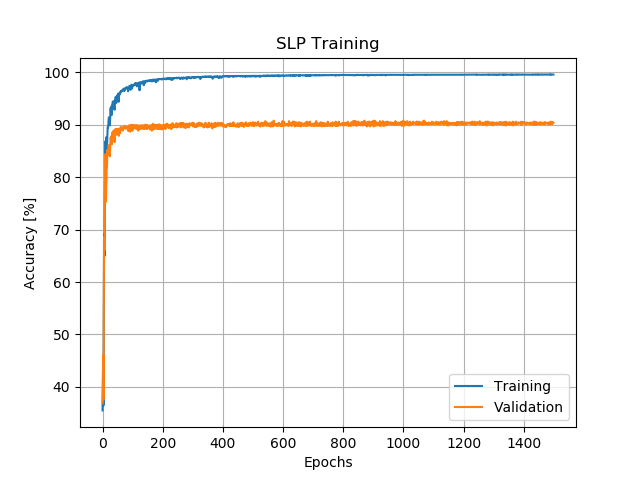
\includegraphics[width=\textwidth]{slp_training.png} % first figure itself
        \caption{SLP Training}
        \label{fig:slp_train}
    \end{minipage}\hfill
    \begin{minipage}{0.45\textwidth}
        \centering
        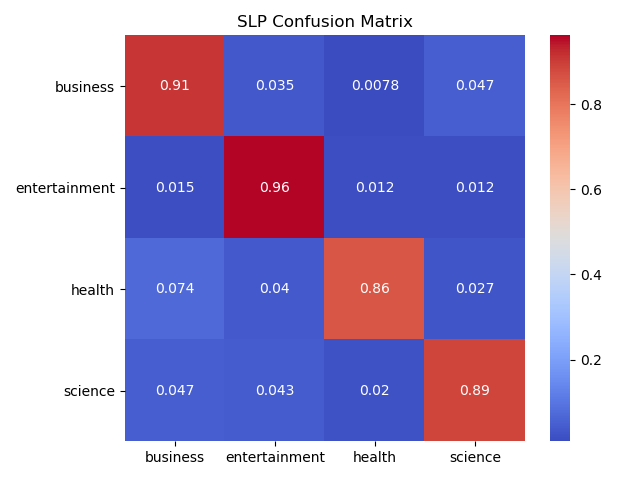
\includegraphics[width=\textwidth]{slp_confmat.png} % second figure itself
        \caption{SLP Confusion Matrix (Test Set)}
        \label{fig:slp_confmat}
    \end{minipage}
\end{figure}
We can see in Figure \ref{fig:slp_train} that the training went quite smoothly and we can confidently say that the model is not overfitting since the training and validation accuracies do not split apart as the epochs progress. The final accuracies we reached are $98.82 \%$ for the training set, $90.5 \%$ for the validation one and $91.5 \%$ for the test set, which is only a $0.4 \%$ increase upon the Bayesian Classifier.  
\subsection{Multi-Layer Perceptron}
The \textit{Multi-Layer Perceptron} was the best performing but the most challenging to tune. We tested multiple architecture and we found that the better performing ones were the ones with only one hidden layer, if we added more the models would overfit. Once we settled on a one hidden layer model we tested various width, results of those tests can be seen in Figure \ref{fig:mlp_test}.
\begin{figure}[!ht]
\centering
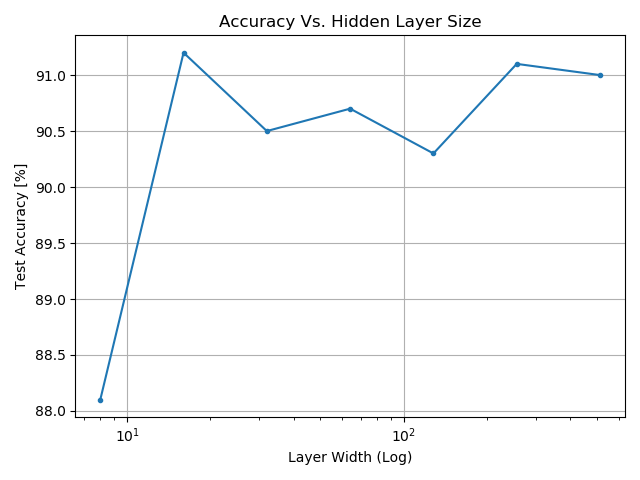
\includegraphics[width=0.5\linewidth]{mlp_tests.png}
\caption{MLP width tests}
\label{fig:mlp_test}
\end{figure}
We decided to take the penultimate point on the graph, corresponding to a width of $256$. We can then represent its architecture with $[8001, 256, 4]$. To train it we used the same parameters used for the SLP, but we trained this model for $350$ epochs since it started to overfit afterwards. 
\begin{figure}
    \centering
    \begin{minipage}{0.45\textwidth}
        \centering
        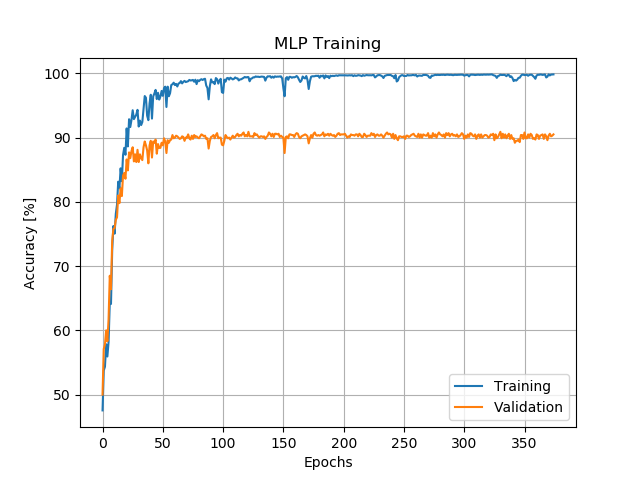
\includegraphics[width=\textwidth]{mlp_training.png} % first figure itself
        \caption{MLP Training}
        \label{fig:mlp_train}
    \end{minipage}\hfill
    \begin{minipage}{0.45\textwidth}
        \centering
        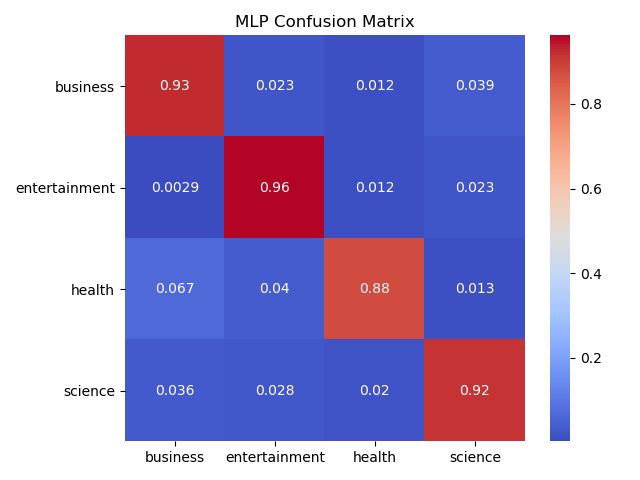
\includegraphics[width=\textwidth]{mlp_confmat.png} % second figure itself
        \caption{MLP Confusion Matrix (Test Set)}
        \label{fig:mlp_confmat}
    \end{minipage}
\end{figure}
The MLP training also went smoothly as we can see in Figure \ref{fig:mlp_train}. The final accuracies reached were $99.1 \%$ on the training set, $90.4 \%$ on the validation one and $92.9 \%$ on the test set.
\section{Results Analysis}
In order to give meaning to the results we obtained we decided to take a look at the confusion matrices of each classifier obtained on the test set. We can see that every classifier struggled the most with the \enquote{health} class, which is curiously mostly confused with the \enquote{business} one. As we expected the Bayesian Classifier confusion matrix is the most noisy, followed by the SLP and MLP. We provided the code with the ability of telling which words are the most influential based on publisher and class (results can be found in the \enquote{most\_polarizing.txt} file) and telling, for each classifier, which titles are wrongly classified with the most confidence (results in the \enquote{wrong} files). With regards to the most influential words we can say that the ones that make the most sense for each publisher are the ones in their belonging classes. For example the most meaningful words for the \enquote{Ubergizmo} publisher are the ones in the science category, as can be inferred from Figure \ref{fig:pub_vs_class}. This confirms that keeping the publisher as a feature was most definitely a good idea. The same titles wrongly classified with the most confidence can be found in each classifier. This gives them more credibility since they struggle to classify the same titles. We also tried a human test, we took the $5$ most misclassified titles of MLP and hid the correct classes. We then asked a human (our sister) to classify them. It turns out that she can beat our classifier since she got $3/5$ right. After this test thought we started to suspect that some items in the dataset might be misclassified, we can hardly agree on the classification of said items. For example we would not classify \enquote{Behind Alibaba IPO is an unlikely China success story} or \enquote{UPDATE 1-Twitter buys social data provider Gnip, stock soars} as \enquote{science}, we would put them in the \enquote{business} category. In other cases we can see why the classifiers make a mistake, such as \enquote{Transformers: Age of Extinction Brings Giant Robot Dinosaurs and Even Bigger  ...} which is understandably classified as \enquote{science} instead of \enquote{entertainment}.     
\section{Conclusions}
The \textit{Multinomial Naive Bayesian Classifier} set a very high baseline to beat. As expected though the \textit{SLP} and \textit{MLP} were able to beat it. We would not recommend the \textit{Logistic Regression} since it not only underperformed with respect to the others but it also took forever to train. We can take a look at Figure \ref{fig:acc_time}\footnote{The radius of the bubbles is proportional to the number of epochs the model was trained for. In the Bayesian case we arbitrarily choose a value lower than all the others since we cannot properly speak of epochs in its training.} too see how much it took to train the various models and their final test accuracy.
\begin{figure}[!ht]
\centering
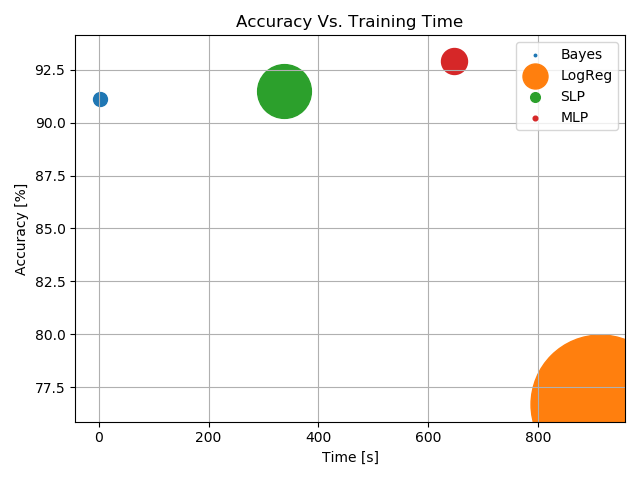
\includegraphics[width=0.5\linewidth]{acc_vs_time.png}
\caption{Accuracy vs. Time}
\label{fig:acc_time}
\end{figure}
In conclusion we can say that we would use the MLP in a real world task scenario since it was the best performer and did not require an unbearable training time. We think that it could be improved by fine tuning the parameters, given the results of the human test. Anyway we think that its accuracy might be higher that what we calculated given that the hypothesis that some data points are misclassified is true.
\end{document}